\section{Project Management}
\sloppy

\subsection{Project Activity Timeline}

\subsubsection{Phase 1: Problem Formulation and Requirement Analysis}
\paragraph{Status:}Completed
This foundational phase has been successfully concluded, establishing the theoretical framework for the project.
\begin{itemize}
    \item \textbf{Literature Review and Background Research:} A systematic review was conducted covering geometric VINS frameworks (OpenVINS, ORB-SLAM3) and Deep Learning-based approaches (SuperPoint, Deep-UAV SLAM).

    \item \textbf{Gap Identification and Problem Statement:} The research identified critical gaps in existing solutions, specifically regarding performance in low texture, low light environments and the computational demands on edge hardware.
    
    \item \textbf{Requirement Gathering:} Functional requirements for real-time localization and non-functional requirements for low-latency processing were defined, guiding the architectural choices.
    
    \item \textbf{Project Proposal Development:} The formal project proposal, outlining the system architecture (ROS 2 nodes, VIO Bridge) and evaluation metrics (ATE, RPE), was prepared and approved, serving as the blueprint for the current implementation phase.

\end{itemize}

\subsubsection{Phase 2: Resource Gathering}
\paragraph{Status:}Completed
All necessary hardware and software environments have been procured and configured.

\begin{itemize}
    \item \textbf{Model Selection:} After reviewing various algorithms (including OpenVINS and PyCuVSLAM), ORB-SLAM3 was selected as the core visual-inertial odometry framework due to its superior global consistency and support for tightly coupled fusion.

    \item \textbf{Dataset Acquisition:} Obtained benchmark datasets (e.g., EuRoC MAV, KITTI) for algorithm testing and training.

    \item \textbf{Hardware Resource Gathering:} The hardware platform has been finalized and assembled, featuring the specific companion computer (e.g., Jetson Orin/Nano as referenced) and flight controller setup.

    \item \textbf{Tool and Platform Setup:} The software stack has been fully deployed. This includes the configuration of ROS 2 (Humble/Foxy) for inter-process communication, PX4 Autopilot for flight control, and the integration of MAVROS to bridge the high-level VIO data with the low-level flight controller.
\end{itemize}

\subsubsection{Phase 3: Model Evaluation}
\paragraph{Status:}Completed
The selected model has undergone rigorous evaluation to ensure it meets the project's performance criteria.

\begin{itemize}
    \item \textbf{Platform-Based Testing:} ORB-SLAM3 has been implemented and tested within the system architecture. The processing pipeline, including feature extraction and local mapping threads, has been validated.

    \item \textbf{Performance Analysis:}  The system's ability to handle sensor data acquisition and processing has been confirmed. Key configuration parameters for the RGB-D Inertial processing pipeline have been tuned.
\end{itemize}

\subsubsection{Phase 4: Drone Integration}
\paragraph{Status:}Ongoing
The project is currently focused on this critical phase, bridging the gap between software algorithms and physical flight control.

\begin{itemize}
\item \textbf{Drone Assembly and Implementation:} Assemble the drone hardware (frames, motors, sensors, communication modules) and integrate all electronic components. Ensure proper wiring, power distribution, and mechanical stability before software integration.
\item \textbf{Algorithm Implementation:} The VIO Bridge node has been successfully developed to handle frame transformations (Camera Frame to Body Frame) and data conversion between the ROS 2 navigation stack and the PX4 flight
\item \textbf{VINS and Flight Controller Integration:} Interface the VINS output with the drone’s flight control system (e.g., PX4, ArduPilot) so that navigation decisions are directly informed by visual-inertial data.
\item \textbf{Flight Testing:} Conduct a series of indoor and outdoor test flights in different conditions: 
    \begin{itemize}
        \item Low light
        \item High wind
        \item GPS-denied areas
    \end{itemize}
    Record performance metrics and operational stability for further refinement.
\end{itemize}

\subsubsection{Phase 5: Model Improvements and Drone Swarm Exploration}
\paragraph{Status:}Pending
Once a working prototype is validated, efforts shift toward improving robustness and extending functionality to swarm scenarios.

\begin{itemize}
    \item \textbf{Limitation Analysis:}  Currently analyzing flight logs to diagnose critical integration issues, specifically yaw misalignment between the VIO estimate and the flight controller's compass, and coordinate frame discrepancies (FLU vs. NED)
    \item \textbf{System Optimization:} Immediate efforts are focused on resolving SLAM initialization failures caused by lack of motion and mitigating "SLAM Reset" events to ensure continuous, smooth trajectory tracking before autonomous flight.
    \item \textbf{Deep Learning Based Optimizations:} Research is ongoing for Deep Learning based optimizations for ORB-SLAM3 computer vision pipeline to address its limitations in lowlight, low texture environments, and to divide workload between CPU and GPU in the Jetson Orin NX.
\end{itemize}

\subsubsection{Phase 6: Documentation and Dissemination}
\paragraph{Status:}Ongoing
Final phase ensures that all technical, operational, and research details are preserved and communicated effectively.

\begin{itemize}
    \item \textbf{Technical Documentation:}  actively documenting the system architecture, specifically the VIO Bridge internal logic, ROS 2 TF tree transformations, and the hardware wiring diagrams for the Jetson Orin/Pixhawk integration.
    \item \textbf{Demonstration:} Organize a live or recorded demonstration showing the system’s capabilities in real flight and/or swarm scenarios.
    \item \textbf{Research Publications:} Compile results into conference papers or journal articles to share findings with the academic and professional community.
    \item \textbf{Final Reports:} The final project report, research publication (targeting VINS performance in GPS-denied environments), and the live flight demonstration are scheduled for the final phase of the project timeline.
\end{itemize}

\subsection{Task Allocation and Individual Contribution}

The following table details the individual contributions of each team member across the comleted project phases and Task Allocation for Upcoming Project Phases
\begin{table}[H]
\centering
\scriptsize
\caption{Task allocation among team members for all project phases.}
\resizebox{\textwidth}{!}{%
\begin{tabular}{|p{2cm}|p{4.3cm}|p{4.3cm}|p{4.3cm}|}
\hline
\textbf{Phase} & \textbf{Akindu} & \textbf{Tishan} & \textbf{Rashmi} \\
\hline

\textbf{Phase 1: Problem Formulation \& Requirement Analysis} &
\begin{itemize}[leftmargin=*, topsep=0pt, itemsep=0pt, parsep=0pt, partopsep=0pt]
  \item Conducted literature review on Deep Learning VIO
  \item Analyzed limitations of VIO in low light, low texture environments.
\end{itemize} &
\begin{itemize}[leftmargin=*, topsep=0pt, itemsep=0pt, parsep=0pt, partopsep=0pt]
  \item Reviewed UAV hardware constraints and GPS-denied navigation challenges.
  \item Specified hardware requirements (Jetson Orin NX, Pixhawk).
\end{itemize} &
\begin{itemize}[leftmargin=*, topsep=0pt, itemsep=0pt, parsep=0pt, partopsep=0pt]
  \item Defined the Problem Statement regarding urban canyon navigation.
  \item Conducted literature review on Geometric VINS (OpenVINS, ORB-SLAM3).
\end{itemize} \\
\hline

\textbf{Phase 2: Resource Gathering} &
\begin{itemize}[leftmargin=*, topsep=0pt, itemsep=0pt, parsep=0pt, partopsep=0pt]
  \item Creating a Github organization to host codebase.
  \item Set up initial software environments and dependencies
\end{itemize} &
\begin{itemize}[leftmargin=*, topsep=0pt, itemsep=0pt, parsep=0pt, partopsep=0pt]
  \item Procure, assemble, and calibrate all hardware components including cameras, IMUs, and embedded computers
  \item Set up the development environment in Jetson Orin NX
\end{itemize} &
\begin{itemize}[leftmargin=*, topsep=0pt, itemsep=0pt, parsep=0pt, partopsep=0pt]
  \item assisted in camera calibration protocols.
  \item Prepared dataset tools for benchmarking.
\end{itemize} \\
\hline

\textbf{Phase 3: Model Evaluation} &
\begin{itemize}[leftmargin=*, topsep=0pt, itemsep=0pt, parsep=0pt, partopsep=0pt]
  \item Evaluated ORB-SLAM3, pycuvslam
  \item Created a ROS2 Wrapper for PyCuVSLAM
\end{itemize} &
\begin{itemize}[leftmargin=*, topsep=0pt, itemsep=0pt, parsep=0pt, partopsep=0pt]
  \item Deployed ORB-SLAM3 node within the ROS 2 framework.
  \item Optimized the RGB-D processing pipeline.
\end{itemize} &
\begin{itemize}[leftmargin=*, topsep=0pt, itemsep=0pt, parsep=0pt, partopsep=0pt]
  \item Evaluated openVINS and Quallcomm qVIO using an exsisting drone
  \item Evaluated camera models and stereo and mono setups
\end{itemize} \\
\hline

\textbf{Phase 4: Drone Integration} &
\begin{itemize}[leftmargin=*, topsep=0pt, itemsep=0pt, parsep=0pt, partopsep=0pt]
  \item Conducting indoor flight tests and manual-to-autonomous switching.
\end{itemize} &
\begin{itemize}[leftmargin=*, topsep=0pt, itemsep=0pt, parsep=0pt, partopsep=0pt]
  \item Developed the VIO Bridge node for ROS 2 $\leftrightarrow$ PX4 communication
  \item Implementing Coordinate Frame Transformations (RDF to FLU).
\end{itemize} &
\begin{itemize}[leftmargin=*, topsep=0pt, itemsep=0pt, parsep=0pt, partopsep=0pt]
  \item Integrating Marker-based localization (ArUco/AprilTags) for drift correction.
\end{itemize} \\
\hline

\textbf{Phase 5: Model Improvement \& Swarm Exploration} &
\begin{itemize}[leftmargin=*, topsep=0pt, itemsep=0pt, parsep=0pt, partopsep=0pt]
  \item Augmenting ORB-SLAM3 computer vision pipeline with deep learning based components and testing
\end{itemize} &
\begin{itemize}[leftmargin=*, topsep=0pt, itemsep=0pt, parsep=0pt, partopsep=0pt]
  \item Integrating Enhaced ORBSLAM3 with the drone and HITL Testing
\end{itemize} &
\begin{itemize}[leftmargin=*, topsep=0pt, itemsep=0pt, parsep=0pt, partopsep=0pt]
  \item Implementing algorithmic fixes for initialization failures (stationary start).
\end{itemize} \\
\hline

\textbf{Phase 6: Documentation \& Dissemination} &
\begin{itemize}[leftmargin=*, topsep=0pt, itemsep=0pt, parsep=0pt, partopsep=0pt]
  \item Preparing and Maintaining documentation in repositories
  \item Producing the Video Demonstration of the flight tests.
\end{itemize} &
\begin{itemize}[leftmargin=*, topsep=0pt, itemsep=0pt, parsep=0pt, partopsep=0pt]
  \item Documenting Software Architecture, VIO Bridge logic, and API references.
  \item Creating Hardware Integration Manuals and wiring diagrams.
\end{itemize} &
\begin{itemize}[leftmargin=*, topsep=0pt, itemsep=0pt, parsep=0pt, partopsep=0pt]
  \item Compiling Documentation
  \item Organize demonstration materials
  \item Prepare publications for academic dissemination
\end{itemize} \\
\hline

\end{tabular}}
\end{table}


\subsection{Summary}
% Shown in the following Table is a summary of project activities in each phase of the project.
% \begin{table}[H]
% \centering
% \small
% \begin{tabular}{|p{3cm}|p{5.5cm}|p{5.5cm}|}
% \hline
% \textbf{Phase} & \textbf{Main Focus} & \textbf{Expected Outcomes} \\ \hline
% 1. Problem Formulation & Define problem, requirements, proposal & Clear problem statement, project proposal, defined scope \\ \hline
% 2. Resource Gathering & Collect models, datasets, platforms & Ready-to-use algorithms, datasets, and simulation environments \\ \hline
% 3. Model Evaluation & Test and compare VINS models & Performance metrics, best model selected \\ \hline
% 4. Drone Integration & Implement and test VINS on hardware & Functional VINS-enabled drone with tested navigation \\ \hline
% 5. Model Improvement \& Swarm Exploration & Optimize system, extend to swarm & Improved robustness, initial swarm coordination results \\ \hline
% 6. Documentation \& Dissemination & Reporting and sharing findings & Technical documentation, publications, final project report \\ \hline
% \end{tabular}
% \caption{Summary of Methodology Phases with Focus and Expected Outcomes.}
% \end{table}

\begin{figure}[H]
    \centering
    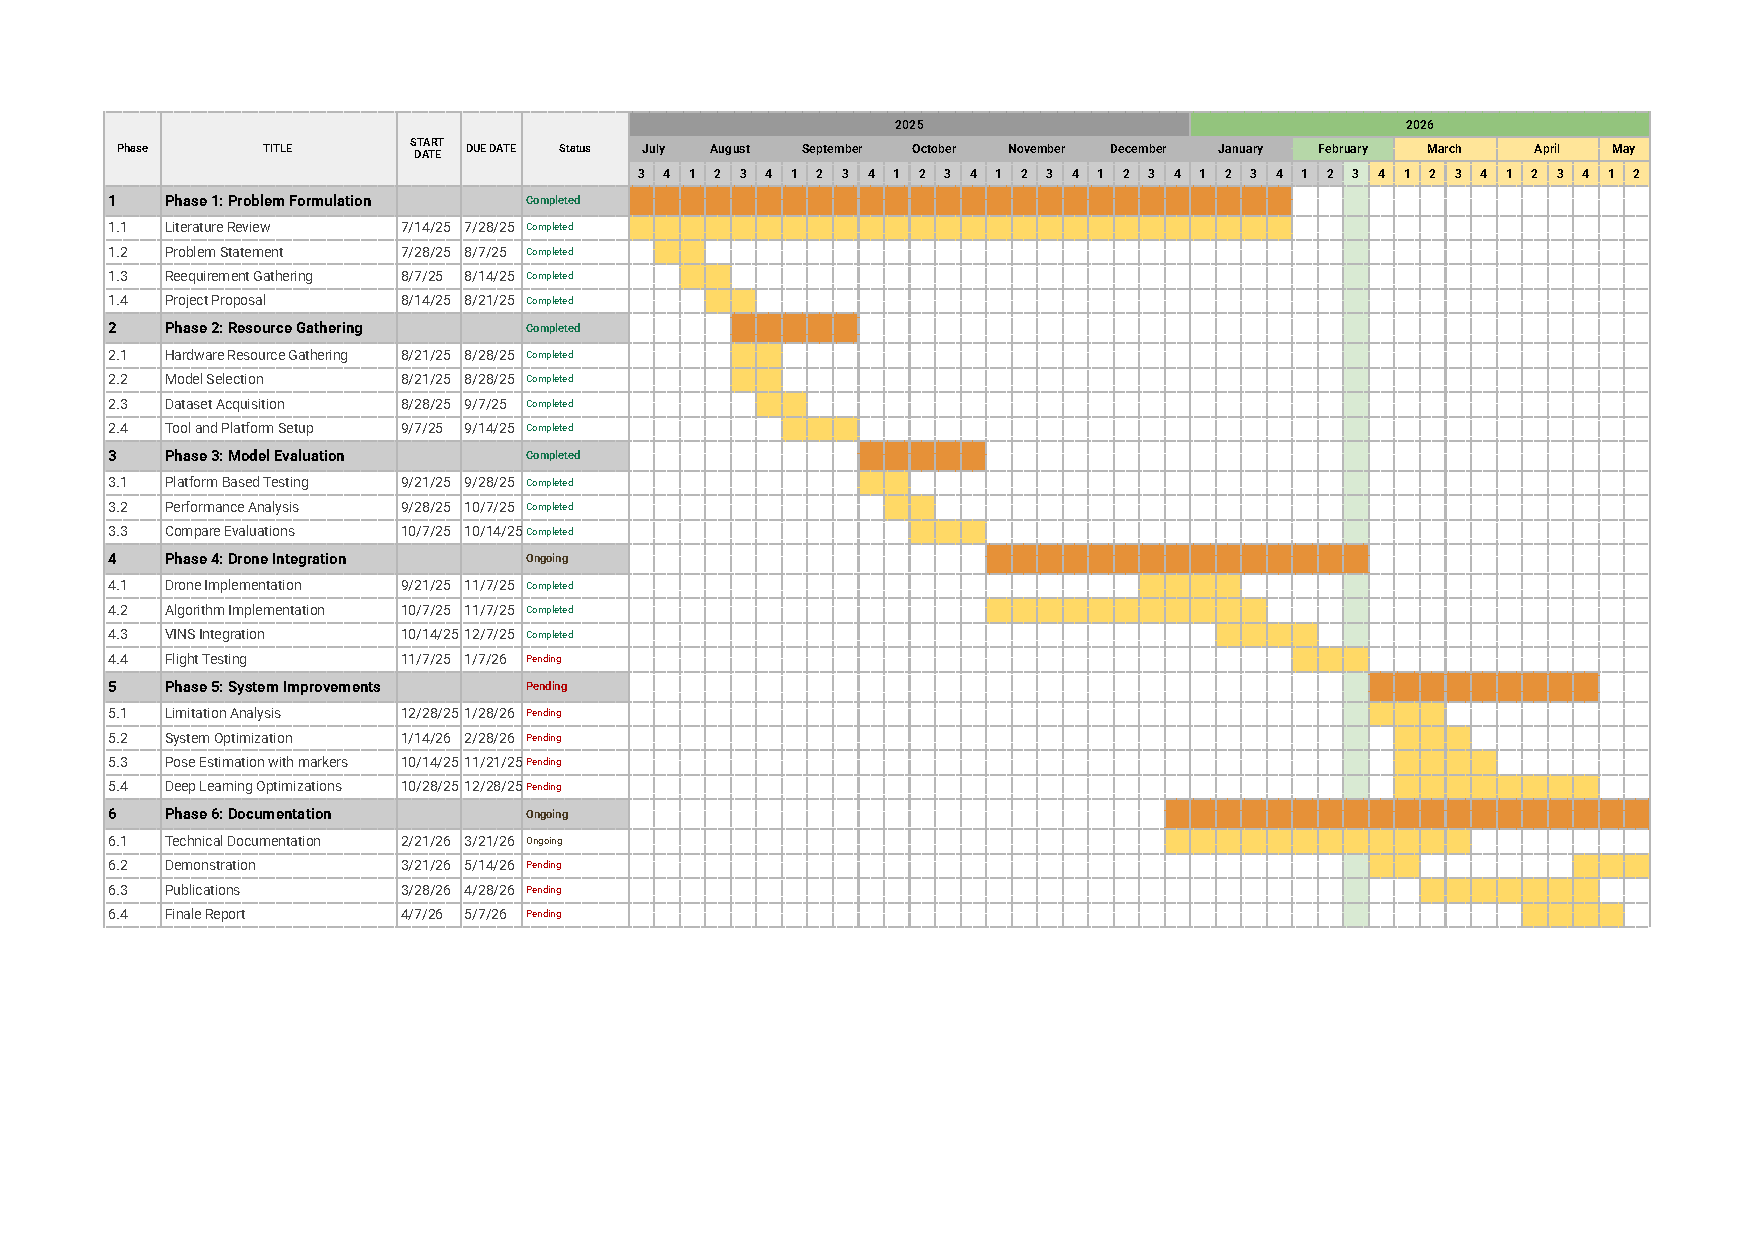
\includegraphics[width=\textwidth, trim=1.6cm 4cm 1.6cm 1.8cm, clip]{images/gantt_chart_2.pdf}
    \caption{Research Timeline}
    \label{fig:gantt_chart}
\end{figure}
